\documentclass{article}
\usepackage{graphicx} % Required for inserting images
\usepackage{float}

\title{Segmentation Report}
\date{March 2024}

\begin{document}

\maketitle

\section{Introduction}
During pregnancy, ultrasound imaging is used to measure fetal biometrics. One of these measurements is the fetal head circumference (HC). The HC can be used to estimate the gestational age and monitor growth of the fetus. The HC is measured in a specific cross section of the fetal head, which is called the standard plane. The dataset for this challenge contains a total of 1334 two-dimensional (2D) ultrasound images of the standard plane that can be used to measure the HC. This challenge makes it possible to compare developed algorithms for automated measurement of fetal head circumference in 2D ultrasound images. 

This report is aimed to design an algorithm that can automatically measure the fetal head circumference given a 2D ultrasound image.
\section{Data Understanding}
The data is divided into a training set of 999 images and a test set of 335 images. The size of each 2D ultrasound image is 800 by 540 pixels with a pixel size ranging from 0.052 to 0.326 mm. The pixel size for each image can be found in the csv files: ‘training\_set\_pixel\_size\_and\_HC.csv’ and ‘test\_set\_pixel\_size.csv’. The training set also includes an image with the manual annotation of the head circumference for each HC, which was made by a trained sonographer. The csv file 'training\_set\_pixel\_size\_and\_HC.csv ' includes the head circumference measurement (in millimeters) for each annotated HC in the training set. All filenames start with a number. There are 999 images in the trainingset, but the filenames only go to 805. Some ultrasound images were made during the same echoscopic examination and have therefore a very similar appearance. These images have an additional number in the filename in between "\_" and "HC" (for example 010\_HC.png and 010\_2HC.png).

The training data labels were modified using OpenCV in python. The ellipses were filled in, as it caused the model to learn to output a filled in ellipse as well. This output was then used to retrieve the values needed for evaluation, using the OpenCV library, again. We chose this method, as training the model on ellipse labels would regularly result in multiple ellipses in the output. It was assumed that the models would achieve better segmentation than just segmenting the ellipse outline. Now, filling in the ellipses resulted in blobs, after which the largest blob was considered the fetal head.

Training data was augmented to provide more training data. This was done by using a maximum rotation range of 0.2, shifting width of 0.05, height shift of 0.05 and zoom range of 0.05. Shearing was not used, as the accurate representation of a fetal head is compromised. Labels were flipped horizontally and newly created pixels which could appear after a rotation or a width/height shift were filled in.
\section{Network Architecture}
\begin{figure}
    \centering
    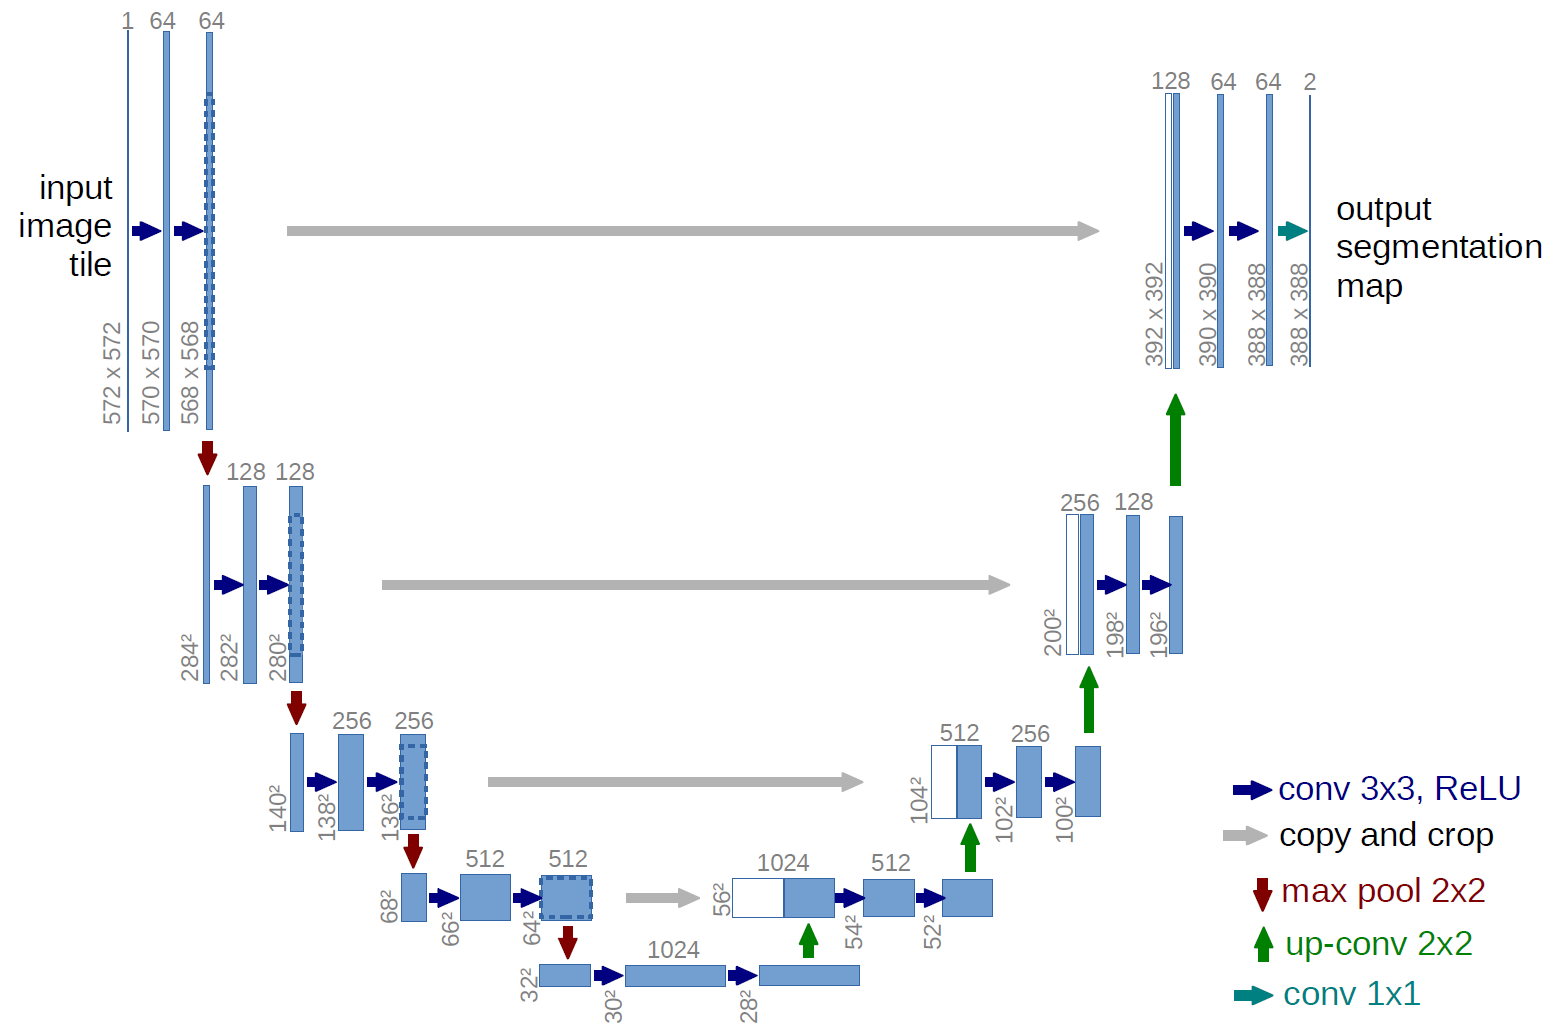
\includegraphics[width=0.8\linewidth]{u-net-architecture.png}
    \caption{U-Net Architecture}
    \label{fig:unet}
\end{figure}
U-net was used for image segmentation of the HC. This is a convolution neural network developed at the Computer Science Department of the University of Freiburg. It is called U-net, as the network architecture is shaped in a ‘U’. This represents the max-pooling layers and up scaling layers in the network, which represent a contracting and expanding path, respectively. This model makes use of valid convolutions. U-net has shown great performance in image segmentation task, such as vessels in the retina, and liver and tumor in CT scans. High performance in these fields led to the implementation of U-net in HC segmentation. In case of our implementation, the Adam optimizer was used, with a learning rate of 1e - 4 The standard binary cross-entropy loss was chosen for optimization. A second (custom) loss function was experimented with as well, to better represent the loss function used in the HC18 Grand Challenge. The discussion provides reasoning for these choices.
\section{Experiment}
\begin{figure}[H]
    \centering
    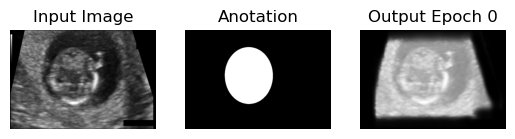
\includegraphics[width=0.8\linewidth]{Unknown-26.png}
    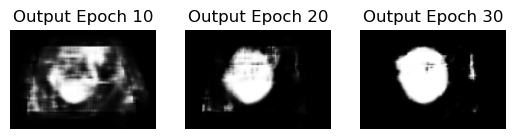
\includegraphics[width=0.8\linewidth]{Unknown-27.png}
    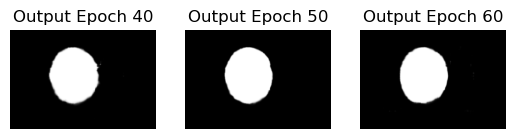
\includegraphics[width=0.8\linewidth]{Unknown-28.png}
    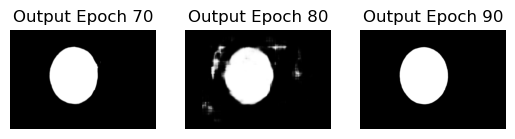
\includegraphics[width=0.8\linewidth]{Unknown-29.png}
    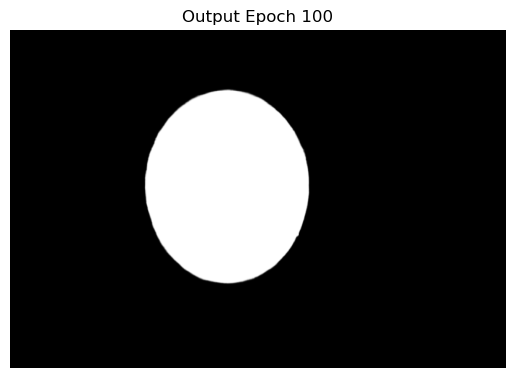
\includegraphics[width=0.8\linewidth]{Unknown-30.png}
    \caption{Outputs of Different Epochs}
    \label{fig:output}
\end{figure}
To preprocess the anotation, we fill it to a full ellipse. We then proceed to train the model for a 100 epochs. The output of each epoch is shown in Fig.\ref{fig:unet}, with the loss progression shown in Fig.\ref{fig:loss}
\begin{figure}[H]
    \centering
    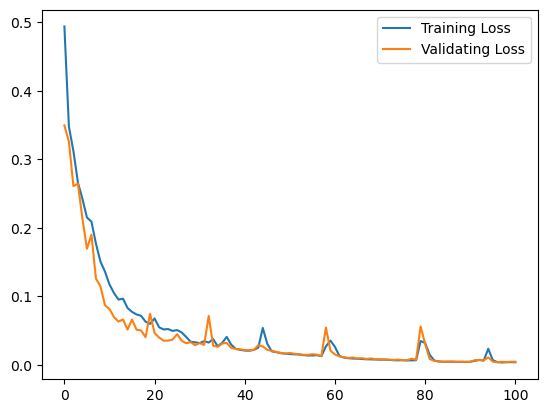
\includegraphics[width=0.7\linewidth]{Unknown-31.png}
    \caption{Training and Validating Loss Progression}
    \label{fig:loss}
\end{figure}
\end{document}
